\documentclass{beamer}
%\usetheme{Ilmenau}
%\usecolortheme{beaver}

\usepackage[slovak,american]{babel}
\usepackage[utf8]{inputenc}
\usepackage{graphicx}
\usepackage{adjustbox}
 \usepackage{xcolor}
 
 \newsavebox\MBox
\newcommand\Cline[2][red]{{\sbox\MBox{$#2$}%
  \rlap{\usebox\MBox}\color{#1}\rule[-2.2\dp\MBox]{\wd\MBox}{1pt}}}

%\usefonttheme{serif}

\definecolor{UKOrange}{HTML}{ef9424} %
\definecolor{UKBrown}{HTML}{a96d5e} %
\definecolor{UKLight}{HTML}{d8b6ab} %
\definecolor{UKDark}{HTML}{7a4f44}
\definecolor{UKDarker}{HTML}{4d312b} 
\definecolor{UKDarkest}{HTML}{2e1e1a}
\definecolor{UKRed}{HTML}{bf1f1c}

\setbeamertemplate{footline}[frame number]{}
\setbeamertemplate{navigation symbols}{}

%\usecolortheme{beaver}
\setbeamertemplate{itemize item}[square]
\setbeamercolor{itemize item}{fg = UKBrown}
\setbeamercolor{itemize subitem}{fg = UKLight}
\setbeamercolor{enumerate item}{fg = UKDark}

\setbeamercolor{footnote}{fg=UKLight}
\setbeamercolor{footnote mark}{fg=UKLight}
\setbeamerfont{footnote}{size=\tiny}
\renewcommand\footnoterule{}

\usetheme{default}
\beamertemplatenavigationsymbolsempty
\setbeamercolor{title}{fg=white, bg=UKBrown}
\setbeamercolor{frametitle}{fg=white, bg=UKBrown}
\setbeamercolor{block title}{bg=UKBrown, fg= white}
\setbeamercolor{block body}{bg =UKLight, fg = UKDarkest}

\useoutertheme[subsection=false]{miniframes}
\AtBeginSection[]{\subsection{}}

\setbeamercolor{below lower separation line head}{bg=UKDark}
\addtobeamertemplate{headline}{}{%
  \begin{beamercolorbox}[colsep=0.5pt]{below lower separation line head}
  \end{beamercolorbox}
}
%\setbeamercolor*{mini frame}{fg=white,bg=UKRosy}
\setbeamercolor{section in head/foot}{fg=UKLight, bg=UKDark}

%\setbeamertemplate{itemize/enumerate body begin}{\normalsize}
%\setbeamertemplate{itemize/enumerate subbody begin}{\normalsize}




%\newcommand{\codeblock}[2]{ \begin{block}{#1} \begin{verbatim}#2\end{verbatim}\end{block}}

%\defbeamertemplate*{title page}{customized}[1][]
%{
%  \begin{centering}
%    \begin{beamercolorbox}[sep=8pt,center]{title}
%      \usebeamerfont{title}\inserttitle
%    \end{beamercolorbox}
%  \end{centering}
%  \bigskip
%
%\begin{columns}[onlytextwidth,T]
%
%
%  \column{27mm}
%  \includegraphics[width=27mm]{images/logoFMFI.png}
%  
%  \column{\dimexpr\linewidth-54mm-6mm}
%  \centering
%  \vspace{5mm}  
%  \usebeamerfont{author}\insertauthor\par
%  \vspace{5mm}
%  \usebeamerfont{institute}\insertinstitute\par
%
%  \column{27mm}
%  \includegraphics[width=27mm]{images/logoUK.png}  
%\end{columns}
%\centering
%\vspace{7mm}
%  \usebeamerfont{date}\insertdate\par
%}

\DeclareMathOperator*{\argmax}{arg\,max}


\title[Validácia, Stromy]{Rozpoznávanie obrazcov - 10. cvičenie \\ Rozhodovacie stromy}
\author[Viktor Kocur]{Viktor Kocur \\{\small viktor.kocur@fmph.uniba.sk}}
\institute{DAI FMFI UK}
\date{27.4.2020}
%\titlegraphic{\includegraphics[width=2.7cm]{images/logoFMFI.png}\hspace*{1cm}~%
%   \includegraphics[width=2.7cm]{images/logoUK.png}
%}


\begin{document}
\selectlanguage{slovak}

\begin{frame}[plain]
  \titlepage  
\end{frame}

\section{Vyhodnocovanie klasifikátorov}
\begin{frame}
\frametitle{Vyhodnocovanie}
  \begin{block}{Viacero tried}
  Doteraz sme väčšinou riešili klasifikačné úlohy, v ktorých sme mali zväčša len dve triedy. Niektoré klasifikátory (NB, kNN), ktoré sme skúšali však dokážu klasifikovať do viacero tried. Pre tie ktoré sú z princípu len binárne je možné nakombinovať viacero binárnych klasifikátorov aby sme získali viactriedny klasifikátor.
  \end{block}   
  
  \begin{block}{fitceocc}
  Mdl = fitcecoc(X, y) - vráti multitriednu verziu SVM klasifikátora
  \end{block}   


\end{frame}


\begin{frame}
\frametitle{Presnosť}
\begin{block}{Stačí presnosť?}
Presnosť (accuracy) definujeme ako podiel počtu správne klasifikovaných príkladov s celkovým počtom príkladov. Takáto metrika na klasifikátor však môže zlyhať. Napríklad ak máme v v príkladoch iba 10 \% jednej triedy a 90 \% druhej, tak klasifikátor, ktorý vždy vráti druhú triedu bude mať 90 \% presnosť, ale ja nám jasné, že to nieje dobrý klasifikátor.
\end{block}
\end{frame}


\begin{frame}
\frametitle{Matica zámen}
  \begin{block}{Matica zámen}
  Jeden zo spôsobov ako vyhodnocovať klasifikátor je tzv. matica zámen. Matica má v i-tom riadku a j-tom stĺpci počeť objektov, ktorých sú z triedy i a sú klasifikované ako trieda j.
  \end{block}   

  \begin{block}{confusionmat}
  C = confusionmat(g1,g2) - vráti maticu zámen pre pravé triedy g1 a predikované triedy g2.
  \end{block} 
    
  \begin{block}{confusionchart}
  cm = confusionchart(g1,g2) - rovno nakreslí maticu zámen
  \end{block}         
\end{frame}



\begin{frame}
\frametitle{True/False Positive/Negative}
Budeme teraz operovať s pojmamy vždy pre jednu triedu:
\begin{itemize}
\item True Positive - TP\\ klasifikátor určil, že príklad je z triedy a je to pravda
\item False Positive - FP\\ klasifikátor určil, že príklad je z triedy ale nieje to pravda
\item True Negative - TN\\  klasifikátor určil, že príklad nieje z triedy a je to pravda
\item False Negative - FN \\ klasifikátor určil, že príklad nieje z triedy ale nieje to pravda
\end{itemize}
\end{frame}

\begin{frame}
\frametitle{Precision a Recall}

\begin{block}{Precision}
Presnosť (precision) definujeme ako $\frac{TP}{TP + FP}$. Rozdiel medzi precision a accuracy bežne spočíva v tom, že pri accuracy delíme počtom všetkých príkladov.
\end{block}

\begin{block}{Recall}
Citlivosť (recall) počítame ako $\frac{TP}{TP + FN}$, teda podiel koľko príkladov klasifikátor určil správne zo všetkých ktoré mal určiť.
\end{block}

\begin{block}{Úloha}
Pre dataset fisheriris vytvorte klasifikátor a spočítajte maticu zámen. Spočítajte aj presnosť a citlivosť pre všetky triedy.
\end{block}

\end{frame}


\section{Rozhodovacie stromy}

\begin{frame}
\frametitle{Rozhodovacie stromy}
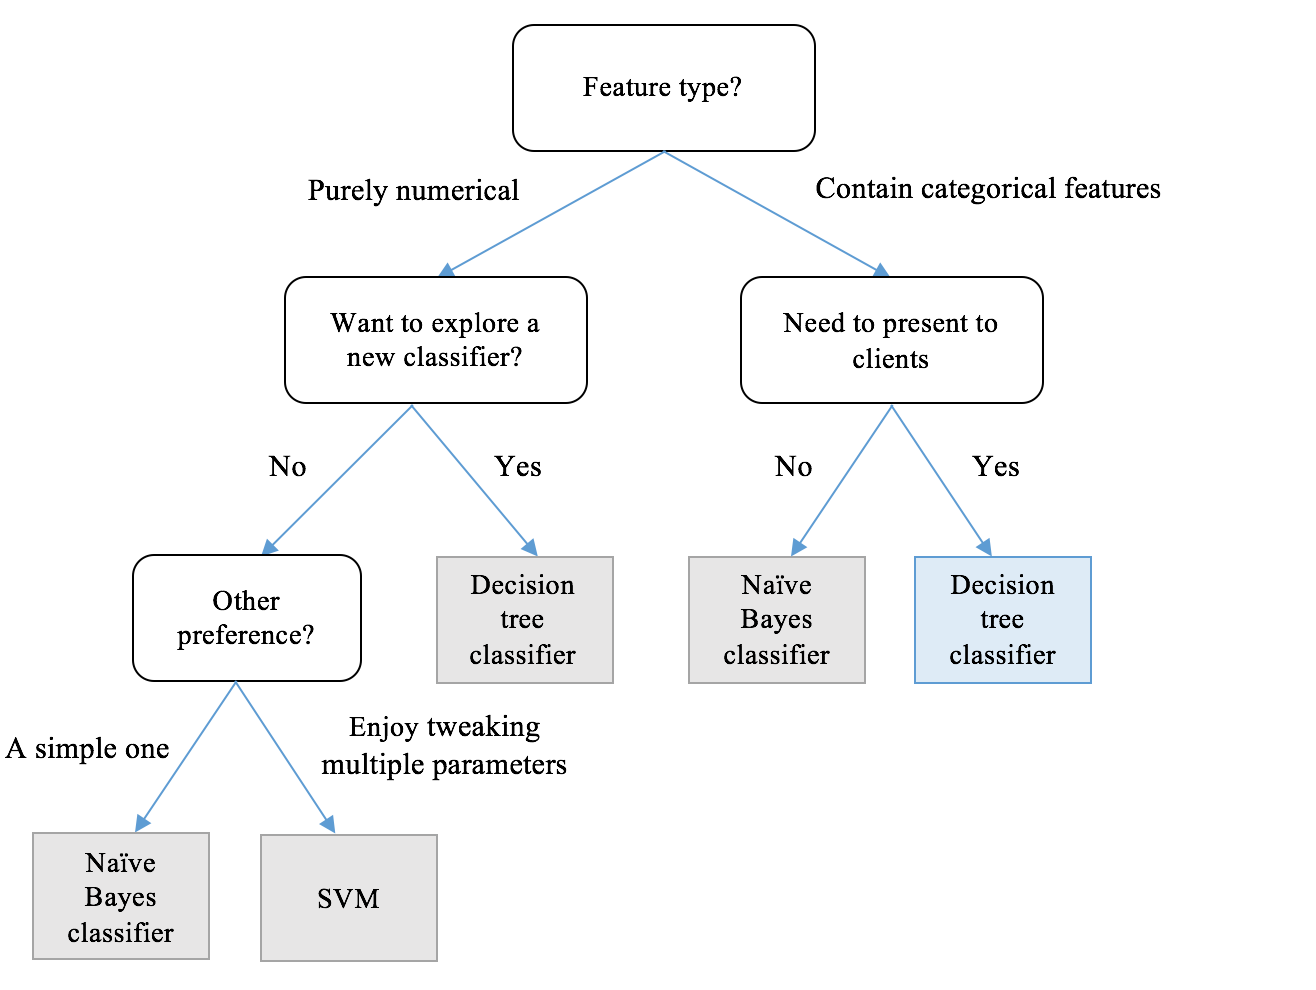
\includegraphics[width=0.9\textwidth]{metatree.png}
\end{frame}

\begin{frame}
\frametitle{Rozhodovacie stromy}
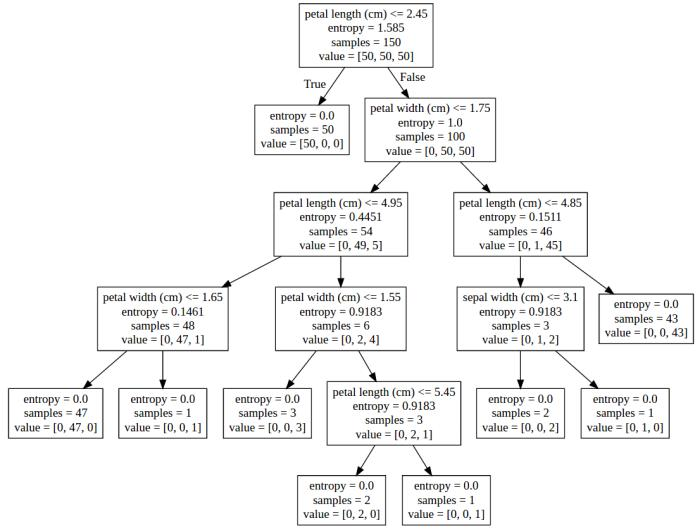
\includegraphics[width=0.9\textwidth]{bettertree.jpg}
\end{frame}


\begin{frame}
\frametitle{Konštrukcia rozhodovacích stromov}

\begin{block}{Rozdelujúce kritérium}
Strom konštruujeme, tak že vyberáme príznak a jeho hodnotu na základe ktorého rozdelíme množinu prvkov na dve časti. Tento postup opakujeme s oboma podmnožinami až kým nieje splnené ukončujúce kritérium.
\end{block}

\begin{block}{Ukončujúce kritérium}
Môže to byť napríklad: podmnožiny obsahujú iba po jednej triede, strom dosiahol nastavenú hĺbku, menší ako prahový počet zle klasifikovaných prvkov v nejakom uzle, ohodnotenie najlepšieho príznaku je menšie ako prah.
\end{block}
\end{frame}

\begin{frame}
\frametitle{Rozhodovacie kritériá}

\begin{block}{ID3}
Vyberáme príznak pre ktorý bude entrópia minimálna, teda taký pre ktorý je informačný prínos najväčší (vzájomná informácia s triedami je najväčšia).
\end{block}

\begin{block}{C4.5}
Obdobne ako pri ID3, ale tentokrát maximaluzujeme normalizovaný informačný prínos. C4.5 navyše dokáže pracovať s numerickými dátami.
\end{block}
\end{frame}


\begin{frame}
\frametitle{Rozhodovacie kritériá - teória zo 4. cvičenia}

\begin{block}{Entrópia}
$$H(Y) = \sum_{y \in \omega} - P(Y = y) \cdot log_2(P(Y=y))$$
\end{block}

\begin{block}{Špecifická podmienená entrópia}
$$H(Y| X = v) = H(Y), \textnormal{len pre hodnoty} Y, \textnormal{kde } X = x $$
\end{block}
\end{frame}


\begin{frame}
\frametitle{Rozhodovacie kritériá - teória zo 4. cvičenia}
\begin{block}{Vzájomná informácia, informačný prínos}
$$I(Y;X) = H(Y) - H(Y|X) = H(Y) - \sum_{x \in \omega} P(X = x)\cdot H(Y|X = x)$$
\end{block}

\begin{block}{Normalizovaný informačný prínos}
$$nI(Y;X) = \frac{I(Y;X)}{H(X)}$$
\end{block}
\end{frame}


\begin{frame}
\frametitle{Príklady}

\begin{block}{ID3}
\url{https://sefiks.com/2017/11/20/a-step-by-step-id3-decision-tree-example/}
\end{block}

\begin{block}{C4.5}
\url{https://sefiks.com/2018/05/13/a-step-by-step-c4-5-decision-tree-example/}
\end{block}
\end{frame}


\begin{frame}
\frametitle{Matlab}
\begin{block}{fitctree}
Mdl = fitctree(X,y) - vráti klasifikačný model rozhodovacieho stromu.
\end{block}

\begin{block}{fitctree}
Mdl = fitctree(T,property) - vráti klasifikačný model rozhodovacieho stromu podľa tabulky T pre klasifikačný ciel v stĺpci property.
\end{block}

\begin{block}{CART}
MATLAB používa metódu CART, ktorá je podobná metóde ID3, ale je mierne iná. Keďže na prednáške nieje, tak ju nebudeme rozoberať.
\end{block}
\end{frame}


\begin{frame}
\frametitle{Matlab}

\begin{block}{predict}
Mdl.predict(x) - vráti predpoveď modelu pre daný príznakový vektor.
\end{block}

\begin{block}{view}
Mdl.view('Mode','graph') - zobrazí strom
\end{block}

\begin{block}{Úloha}
Vytvorte a zobrazte si strom pre databázu fisheriris a census1994. Pre census1994 zistite presnosť.
\end{block}
\end{frame}

\begin{frame}
\frametitle{Orezávanie stromov}
\begin{block}{Orezávanie}
Strom môže byť zbytočne komplikovaný. To vedie na overfitting. Strom je možné orezať tak, že podstromy, ktoré prinášajú zanedbateľné zlepšenie presnosti klasifikácie nahradíme listom.
\end{block}

\begin{block}{prune}
MdlP = prune(Mdl,'Property', value) - vráti orezaný strom podľa toho ako je nastavená property
\end{block}

\begin{block}{Úloha}
Orežte strom pre dáta fisheriris a census1994. Otestujte rôzne properties (Level, Alpha, Nodes) a otestujte zlepšenie presnosti na testovacej množine pre census1994.
\end{block}

\end{frame}




\end{document}